\chapter{四足機器人有限元素分析}

此專題以有限元素法作為主題,四足機器人為載體,目的就是為了使用有限元素法計算載體的受力後狀態,並利用了CoppeliaSim對模型進行了動態模擬,找出了各部件的最大力方向及位置。\
我們將單一步行機構負重定為五倍自身重量,為承受力630N,材質則選用了常見的ABS材料。\
分析環境選擇Solid Edge及Ansys同時進行,以利於對比資料並查看兩軟體區別。\\

%-----------------------有限元素分析--------------------------%
\section{有限元素分析}
\begin{itemize}
\item 下列為個部位進行有限元素分析的步驟介紹
\end{itemize}
\begin{enumerate}
\item 開啟設計模型並開啟Solid Edge分析功能新增研究內容/另存為IGES(.igs)檔案用以匯入Ansys。
\item 材料選擇3D列印機常用的ABS材質,在未來有需求時能夠及時並快速地做實體測驗並打印出模型。
\item 依照原先設計者的參數設定負載為630N,為自身6倍體重。
\item 通過CoppeliaSim找出個部位所受反力點及最大角度。
\item 通過有限元素法出個部位受力狀態。
\item 觀察求解後參數是否符合要求或是需要修改。\\

\end{enumerate}
以上步驟為有限元素法在兩個軟體中通過電腦計算在四足機器狗上的應用,用兩個軟體分析目的為比較之間的算法差異,找出哪種算法更適合其對應模型或是缺陷,以利於後續分析調整中。\
有限元素分析經常會被設計師套用在其設計上,用以尋找產品缺陷或改進。\
\newpage
%-----------------------分析比較--------------------------%
\section{Solid Edge與Ansys分析比較}
將零件同時丟進Ansys、Solid Edge進行分析,並比對結果,雖然兩個分析軟體都設定相同的參數,但可能因為軟體的各項因素導致最終結果有所差異,像是軟體使用的模擬方法、網格生成、材料參數、數值設定等因素。\\

\begin{enumerate}
\item 分析方式:使用的數值模擬方法和算法可能因為不同的數學模型和近似方法有所差異。
\item 網格生成:使用不同的網格生成算法,導致在相同設定下生成不同的網格。
\item 材料參數:即使設定相同的材料,兩個軟體的數據庫所使用的材料特性和邊界條件等參數也可能有所差異。
\item	數值設定:即使設定相同的參數,兩個軟體可能使用不同的預設值或建議值也會造成差異。\\

\end{enumerate}

%-----------------------------------------%
\begin{figure}[hbt!]
\center
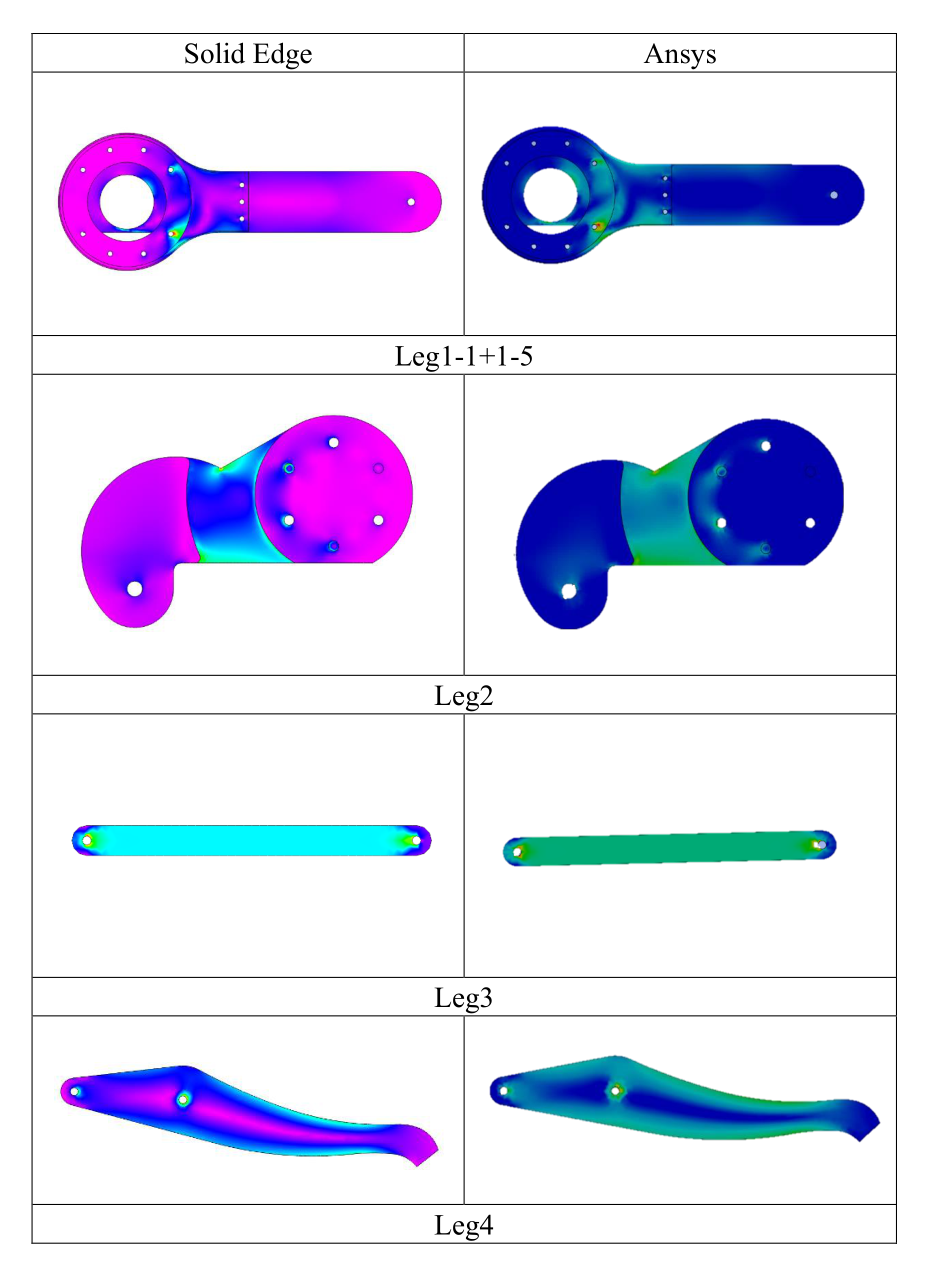
\includegraphics[width=16cm]{分析比對表}
\caption{\Large 分析比對表}
\label{分析比對表}
\end{figure}

\begin{table}[htb!]
  \center\large
  \setlength{\tabcolsep}{0.75cm}{
  \begin{tabular}{|c|c|c|c|c|}
    \hline &Leg1-1+1-5& Leg2 & Leg3 & Leg4  \\
    \hline Solid Edge &68.5 & 28.9 & 15.8 & 57.6  \\
    \hline Ansys &60.7 & 29.2 & 16.1 & 56.7  \\
    \hline
   \end{tabular}}
  \caption{\Large ABS最大等效應力(MPa)}
\end{table}   

得到分析結果後,發現ABS材料在承受五倍自身體重(630N)時,會導致零件最小安全係數未大於等於1,為了符合實際應用,所以將材料換成強度更高的PLA進行分析。\\


\begin{table}[htb!]
  \center
  \large
  \setlength{\tabcolsep}{0.75cm}{
  \begin{tabular}{|c|c|c|c|c|}
    \hline   &Leg1-1+1-5& Leg2 & Leg3 & Leg4 \\
    \hline Solid Edge&69.6 & 30.8 & 15.9 & 61.2  \\
    \hline Ansys &61.2 & 30.0 & 15.8 & 60.5  \\
    \hline
  \end{tabular}}
  \caption{\Large PLA最大等效應力(MPa)}
\end{table}

\begin{table}[htb!]
  \center\large
  \setlength{\tabcolsep}{0.75cm}{
  \begin{tabular}{|c|c|c|c|c|}
    \hline   
    &Leg1-1+1-5& Leg2 & Leg3 & Leg4 \\
    \hline 
    Solid Edge&0.9 & 2.11 & 4.09 & 1.06  \\
    \hline 
    Ansys &1.1 & 2.17 & 4.1 & 1.1  \\
    \hline
  \end{tabular}}
  \caption{\Large PLA最小安全係數}
\end{table}

\newpage
